\section{Measurement and Analysis}
\label{rate-limiter:sec:measurement} \mylabel{sec:measurement}

\wenfei{missing: packet drop measurement.}
\keqhe{say something about why we choose  HTB, just 1 - 2 sentences}

\subsection{Performance of Linux HTB}
\begin{figure}[!t]
\centering
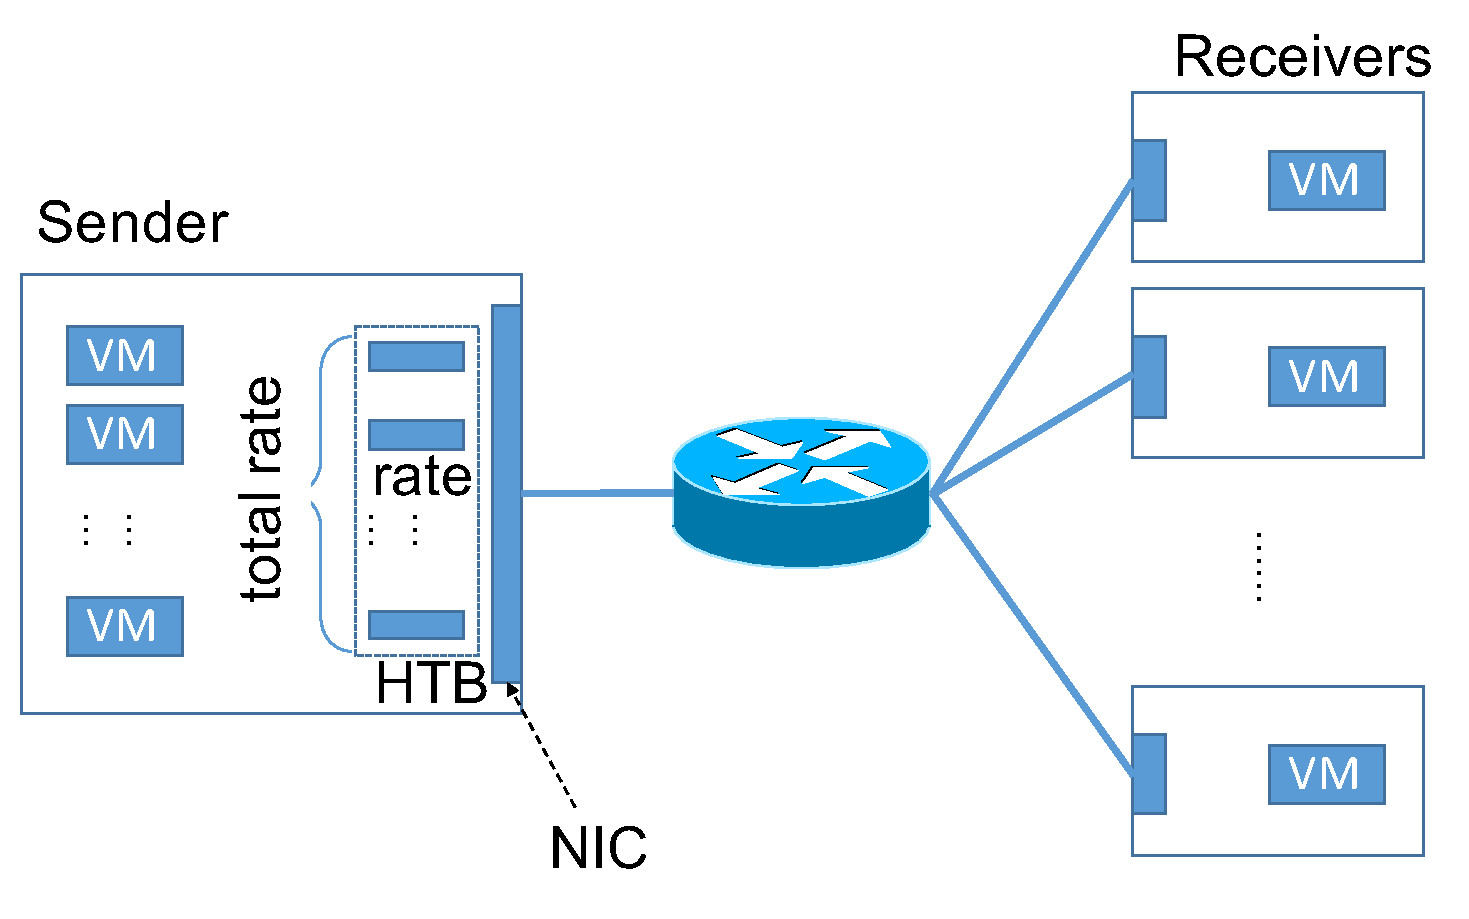
\includegraphics[width=\columnwidth]{figs/exp_setup.pdf}
\caption{Experiment setup}
\label{fig:exp-setup} \mylabel{fig:exp-setup}
\end{figure}


We first measure the performance of Linux HTB rate limiter. 
Compared with other software rate limiters, HTB ensures that a minimum amount of bandwidth is guaranteed 
to each traffic class and
if the required minimum amount of bandwidth is not fully used, the remaining bandwidth is distributed to other classes.
The distribution of spare bandwidth is in proportion to the minimum bandwidth specified to a class~\cite{linux-htb-intro}.
We set up servers in CloudLab, and each server is equipped with 10 Gbps NICs. 
The experiment setup is shown in Figure~\ref{fig:exp-setup}.
%On each server, we configure HTB (the native implementation in Linux 4.2) as software rate limiters. 
In the experiments, we configure a rate limiter for each sender VM; 
for each sender-receiver VM pair, we use iperf to send background traffic. 
We configure HTB to control the bandwidth for each pair, and vary the number of flows between each pair.
We also control the total sending rate of all pairs (i.e., using the hierarchical feature of HTB).
With these settings, we run sockperf between sender and receiver pairs to measure TCP RTT. 
We conducted two sets of experiments. In the first set of experiments, 
we have one sender VM and one receiver VM.
We specify the speed of the sender side rate limiter to 1Gbps, 2Gbps, 4Gbps and 8Gbps. 
We vary the number of iperf flows (1, 2, 8 and 16) from
the sender to receiver. In the second set of experiments, 
we configure two rate limiters on the sender server and set up two VMs (one rate limiter each VM).
We configure the minimum rate of each rate limiter to 2Gbps, 3Gbps, 4Gbps and 5Gbps and
the total rate of the two rate limiters is always 10Gbps. 

\begin{table*}[!tb]
\centering
%\small
{\setlength{\tabcolsep}{1pt}
\begin{tabular}{|l|l|llll|llll|llll|llll|}
\hline
numReceiver          & 1   & 1    & 1    & 1   & 1    & 1    & 1    & 1    & 1   & 1    & 1     & 1      & 1       & 1    & 1    & 1      & 1       \\
numFlows/receiver    & -   & 1    & 1    & 1   & 1    & 2    & 2    & 2    & 2   & 8    & 8     & 8      & 8       & 16   & 16   & 16     & 16      \\
rate/receiver (Gbps) & -   & 1    & 2    & 4   & 8    & 1    & 2    & 4    & 8   & 1    & 2     & 4      & 8       & 1    & 2    & 4      & 8       \\
total rate (Gbps)    & -   & 1    & 2    & 4   & 8    & 1    & 2    & 4    & 8   & 1    & 2     & 4      & 8       & 1    & 2    & 4      & 8       \\
\hline
total tput (mbps)    & -   & 951  & 1910 & 3820 & 7380  & 945  & 1910 & 3820 & 7500 & 958  & 1915  & 3827   & 7627    & 960  & 1920 & 3829   & 7655    \\
b/w saturation (\%)  & -   & 95.1 & 95.5 & 95.5 & 95.3  & 94.5 & 95.5 & 95.5 & 93.8 & 95.8 & 95.8  & 95.7   & 95.3    & 96   & 96   & 95.7   & 95.7 \\
\hline
50\% RTT (us)        & 116 & 957  & 883  & 643 & 1583 & 1513 & 1078 & 1047 & 853 & 2316 & 1766  & 1529   & 1110    & 3192 & 2373 & 1880   & 1262    \\
99.9\% RTT (us)      & 237 & 1115 & 1000 & 706 & 1673 & 1701 & 1203 & 1132 & 933 & 2527 & 1939  & 1637   & 1208    & 3320 & 2511 & 2016   & 1486   \\
\hline
\end{tabular}}
\caption{HTB experiments for one receiver VM}
\label{tbl:htb-1rec} \mylabel{tbl:htb-1rec}
\end{table*}

\begin{table*}[!tb]
\centering
%\small

{\setlength{\tabcolsep}{1pt}
\begin{tabular}{|l|l|llll|llll|llll|llll|}
\hline
numReceiver          & 2   & 2    & 2    & 2    & 2    & 2    & 2    & 2    & 2    & 2     & 2     & 2     & 2     & 2     & 2     & 2     & 2     \\
numFlows/receiver    & -   & 1    & 1    & 1    & 1    & 2    & 2    & 2    & 2    & 8     & 8     & 8     & 8     & 16    & 16    & 16    & 16    \\
rate/receiver (Gbps) & -   & 2    & 3    & 4    & 5    & 2    & 3    & 4    & 5    & 2     & 3     & 4     & 5     & 2     & 3     & 4     & 5     \\
total rate (Gbps)    & -   & 10   & 10   & 10   & 10   & 10   & 10   & 10   & 10   & 10    & 10    & 10    & 10    & 10    & 10    & 10    & 10    \\
\hline
total tput (mbps)    & -   & 9420 & 9420 & 9410 & 9410 & 9410 & 9420 & 9420 & 9420 & 9224  & 9392  & 9321  & 9401  & 9182  & 9161  & 9225  & 9296  \\
b/w saturation (\%)  & -   & 94.2 & 94.2 & 94.1 & 94.1 & 94.1 & 94.2 & 94.2 & 94.2 & 92.2  & 93.9  & 93.2  & 94.0  & 91.8  & 91.6  & 92.3  & 93.0 \\ \hline
50\% RTT (us)        & 118 & 475  & 797  & 1515 & 1658 & 699  & 916  & 1006 & 1036 & 1512  & 1407  & 1410  & 1587  & 2023  & 2040  & 2064  & 1986  \\
99.9\% RTT (us)      & 135 & 551  & 849  & 1626 & 1751 & 983  & 989  & 1102 & 1115 & 1697  & 1673  & 1532  & 1768  & 2147  & 2182  & 2185  & 2100 \\
\hline
\end{tabular}}
\caption{HTB experiments for two receiver VMs}
\label{tbl:htb-2rec} \mylabel{tbl:htb-2rec}
\end{table*}


\begin{figure*}[!htb]
\centering
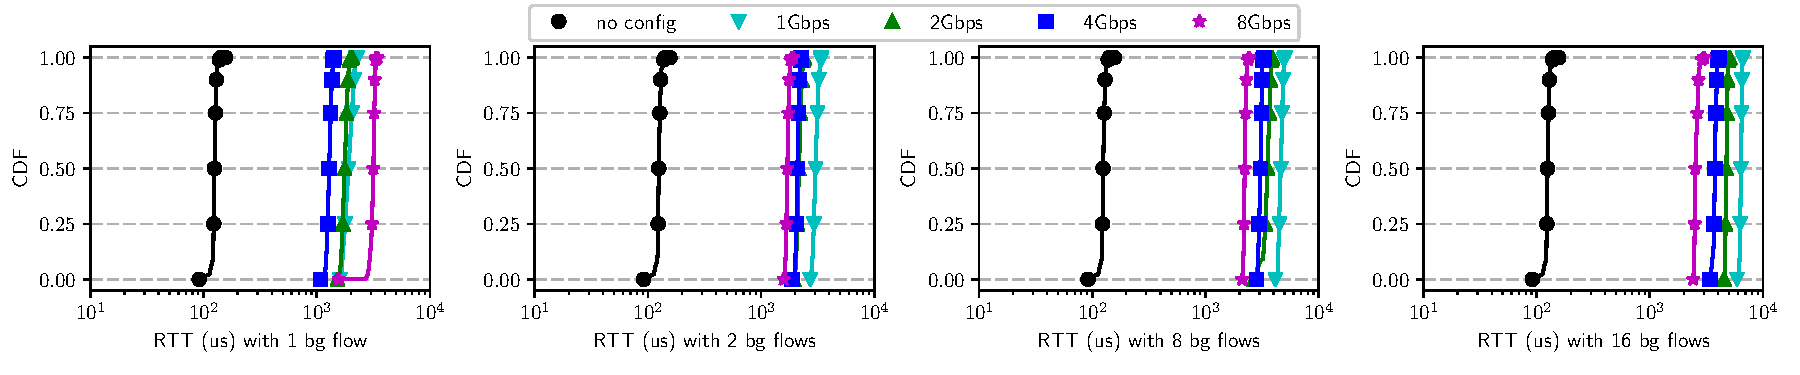
\includegraphics[width=\textwidth]{rate_limiter/raw_data/htb_benchmark/one_receiver.pdf}
\caption{HTB experiment: one receiver VM, varying rate limiting and number of background flows}
\label{fig:htb-1rec} 
\end{figure*}

\begin{figure*}[!htb]
\centering
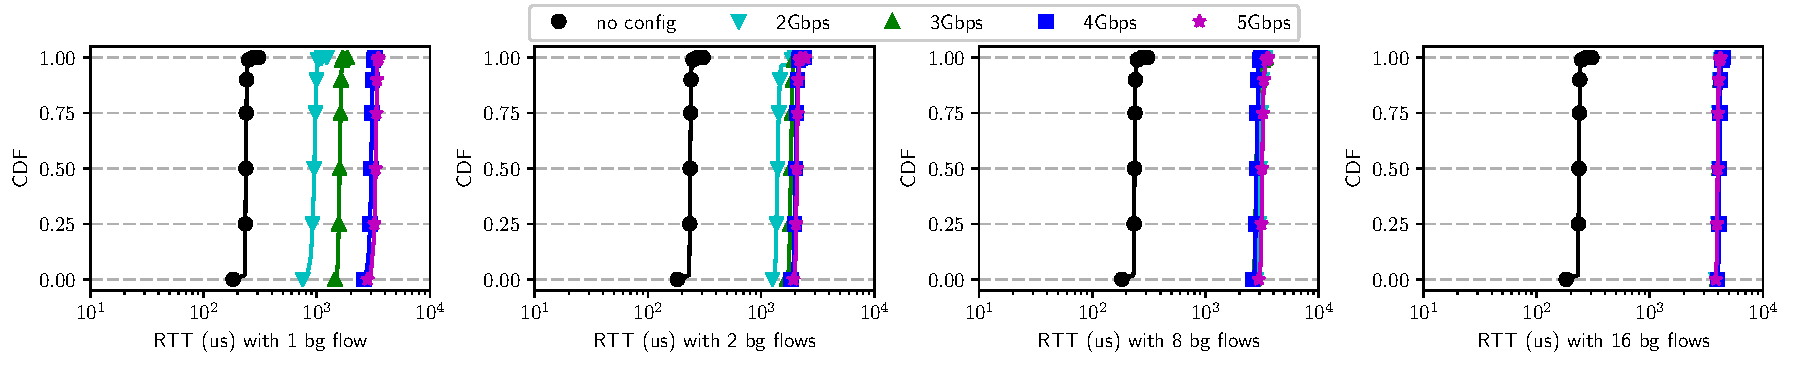
\includegraphics[width=\textwidth]{rate_limiter/raw_data/htb_benchmark/two_receivers.pdf}
\caption{HTB experiment: two receiver VMs, varying rate limiting and number of background flows}
\label{fig:htb-2rec} 
\end{figure*}



The experiments results are shown in Table~\ref{tbl:htb-1rec} and~\ref{tbl:htb-2rec}. 
In all experiment scenarios, network saturation ratio is from 91\%-96\%. 
Note that in Table~\ref{tbl:htb-2rec}, if the sum of individual rate limiter's rate is smaller than the configured total rate, 
HTB would allow all flows to utilize and compete for the spare bandwidth. 
Another observation is that more flows lead to lower bandwidth saturation, 
because there is more competition between flows, which leads to throughput oscillation.

We further look into the scenario of one receiver VM. 
We visualize the TCP RTT results in Figure~\ref{fig:htb-1rec}; each subfigure shows 
the CDF of sockperf trace RTT with different rate limiter speed. 
Different subfigures show scenarios with a varying number of background iperf flows. 
We can draw three conclusions based on the measurement data. First, TCP RTT increases dramatically when packets go through 
a congested rate limiter. 
In the baseline case where no HTB is configured and no iperf background flow running, the median TCP RTT is 62us. 
While with one background iperf flow and rate limiter speed from 1Gbps to 8Gbps, 
the median RTT increases to 957us-1583us, which is 15-25X larger compared with the baseline case. 
Second, TCP RTT increases with more background flows running. For example, 
with 1Gbps rate limiting, the median RTT is 957us for one background flow and 3192us for 16 background flows. 
Third, TCP RTT decreases with larger rate limiter speed 
configured~\footnote{The only exception is the case with one background flow and 
8Gbps rate limiting, which is suspected to be experiment noise.}. 
Because rate limiter speed determines the dequeue speed of HTB queue, thus, with larger dequeue speed, 
the queue tends to be drained faster. 

In the experiments with two receiver VMs (Figure~\ref{fig:htb-2rec}), we can draw the same conclusions regarding RTT increase 
and the impact of the number of background flows. The difference is that TCP RTT increases with 
larger rate limiting speed configured. In these experiments, we did not constrain the total rate, 
allowing HTB to utilize spare bandwidth. Thus, the dequeue speed is constant in each figure (10Gbps/numFlow). 
The possible reason for the trend is that enqueue speed is higher when rate limiter speed is higher.
For a fixed dequeue speed, larger enqueue speed implies higher latency.

\subsection{Strawman Solution: DCTCP + ECN}
\begin{figure*}[!htb]
\centering

\begin{subfigure}[b]{0.45\textwidth}
\centering
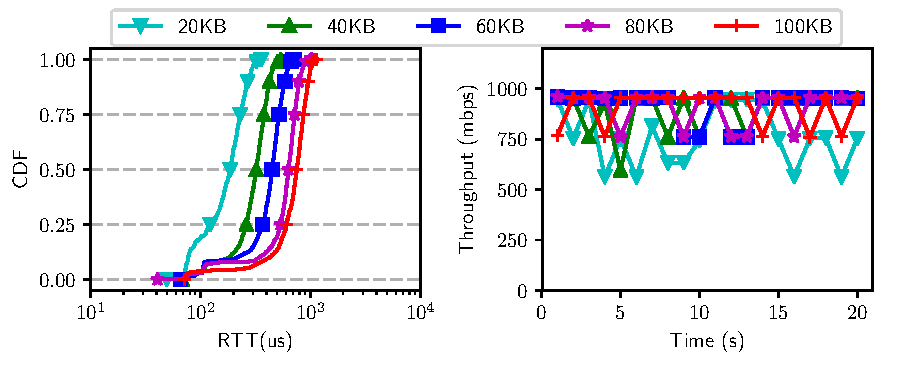
\includegraphics[width=\textwidth]{rate_limiter/raw_data/dctcp_benchmark/1gbps.pdf}
\caption{Rate Limiting: 1Gbps}
\label{fig:dctcp-1g} 
\end{subfigure}
\begin{subfigure}[b]{0.45\textwidth}
\centering
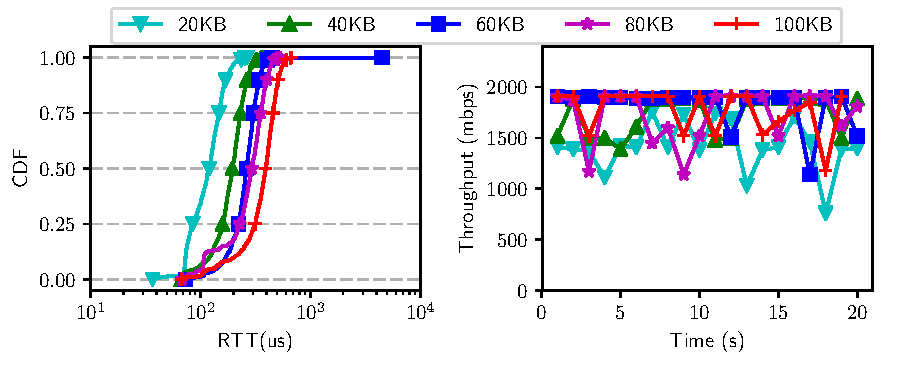
\includegraphics[width=\textwidth]{rate_limiter/raw_data/dctcp_benchmark/2gbps.pdf}
\caption{Rate Limiting: 2Gbps}
\label{fig:dctcp-2g} 
\end{subfigure}
\caption{DCTCP experiments, 1 flow, varying threshold}
\label{fig:dctcp}
\end{figure*}



Inspired by solutions to reduce queueing latency in switches~\cite{alizadeh2010data}, 
we test a strawman solution. In the strawman solution, 
we implement ECN marking in Linux HTB queues and enable DCTCP at the end-points. 
For ECN marking, there is a tunable parameter \textemdash\xspace \textit{marking threshold}. 
When the queue length exceeds the marking threshold, 
all enqueued packets would have their ECN bits set; otherwise, packets are not modified. 
DCTCP reacts to ECN marking and adjusts sender's congestion window based on the ratio of marked packets~\cite{alizadeh2010data}.

We set up experiments with one sender and one receiver. We configure the HTB rate limiter to be 1Gbps and 2Gbps, 
and vary ECN marking threshold. The experiment results are shown in Figure~\ref{fig:dctcp}. 
We observe that TCP RTT can be reduced significantly (<1ms) by extending ECN into rate limiter queues. 
For example, with the marking threshold set to 60KB, median TCP RTT is 224us (Figure~\ref{fig:dctcp-1g}), 
which is less than 1/4 of native HTB's (957us). A smaller ECN marking threshold 
can achieve even lower latency \textemdash\xspace with the threshold from 100KB to 20KB, median TCP RTT is reduced from 375 us to 93us.

While latency can be improved, we observe a negative effect of DCTCP+ECN on the throughput, as shown in Figure~\ref{fig:dctcp}.
TCP throughput appears to have large oscillation, 
which implies applications cannot get constantly high throughput and the bandwidth is not fully utilized. 
For example, with 2Gbps rate limiting (Figure~\ref{fig:dctcp-2g}), 
even we set the threshold to be 100KB (much larger than the best theoretical value according to~\cite{alizadeh2010data}), 
there is still occasional low throughput (e.g., 1000Mbps) within a 20-second experiment duration.

\subsection{Throughput Oscillation Analysis}
Directly applying the existing ECN marking technique to rate limiter queue 
causes TCP throughput oscillation. There are two reasons. First, end-host networking stacks 
enable optimization techniques such TSO (TCP Segmentation Offload~\cite{tcp-segment-offload}) to 
improve throughput and reduce CPU overhead. Therefore, end-host networking stack 
(including the software rate limiters) processes TCP segments instead of MTU-sized packets. 
The maximum TCP segment size is 64KB by default. A TCP segment's IP header is copied 
into each MTU-sized packet in the NIC using TSO. So marking one TCP segment in the rate limiter queue 
results in a bunch of consecutive MTU-sized packets to be marked.
For example, marking a 64KB segment means 44 consecutive Ethernet frames are marked. 
Such coarse-grained segment-level marking finally causes the accuracy of congestion estimation in DCTCP to be greatly decreased. 

Second, ECN marking happens on the transmitting path, and it takes one RTT for 
congestion feedback to travel back to the sender before congestion control actions are taken. 
Moreover, TCP RTT can be affected by the ``in network" latency. ``In network" latency can be milliseconds or tens of milliseconds. 
Thus, this one RTT control loop latency 
would cause the ECN marks to be ``outdated'', not precisely reflecting the instantaneous queue length 
when the marks are used for congestion window update in DCTCP.
Without congestion control based on instantaneous queue length, 
the one-RTT control loop latency exacerbates the incorrect segment-level ECN marking. 
Thus, congestion window computation in DCTCP tends to change more dramatically, leading to the throughput oscillation.


\subsection{Call for Better Software Rate Limiters}

\begin{table}[!tb]
\begin{center}
\begin{tabular}{ |c|c|c|c| }
 \hline
 R1  & high throughput   \\
 R2 & low throughput oscillation  \\
 R3 & low latency \\
 R4 & generic\\
 \hline
\end{tabular}
\caption{Design requirements}
        \label{rate-limiter-design-requirements}
\end{center}
\end{table}

\begin{table}[!tb]
\begin{center}
\begin{tabular}{ |c|c|c|c| }
 \hline
  & Stable Tput & Low Latency & Generic \\
 \hline
 Raw HTB  & \cmark & \xmark & \cmark   \\
 DCTCP+ECN & \xmark & \cmark & \xmark  \\
 \hline
\end{tabular}
\caption{Raw HTB and DCTCP+ECN can not meet the design requirements}
        \label{cannot-meet-design-requirements}
\end{center}
\end{table}

\iffalse
Having observed the flaws of Linux native HTB and the strawman solution, 
it is challenging to achieve both \textit{high throughput and low latency} for rate limiters. They are as follows.

\textbf{\#1. Low oscillation.} As is shown in the strawman solution, achieving requirement \#1 would lead to oscillation in throughput. Thus, the solution should overcome this flaw, i.e., achieving low oscillation.

\textbf{\#2. Generic.} Another weakness of the strawman solution is that it requires the end host to support ECN compatible congestion (e.g., DCTCP). While in clouds, the TCP configuration is not always within the cloud operators' control. So the solution should be generic to be applied to any TCP invariants in tenants' VMs. 

Fortunately, software rate limiters are implemented on end host, which give opportunities to overcome the challenges. First, end host has enough memory to store per-flow information, so that we can store per-flow queue information and correlate the incoming an ACK with its outgoing queue length. Second, in end host kernel, we have sufficient programmability (e.g., loadable OVS module), so we can compute per-flow window size and encode it in packets before they arrive at VMs.
\fi

We list the design requirements for better software rate limiters, as shown in Table~\ref{rate-limiter-design-requirements}. 
First the rate limiter should be able to provide high network throughput. 
Second, network throughput should be stable with low oscillation. 
Third, flows traversing the rate limiter should experience low latency. 
Finally, the rate limiter can be able to handle various kinds of traffic \textemdash\xspace ECN-capable and non ECN-capable. 
Neither raw HTB nor HTB with DCTCP+ECN can meet the four design requirements (see Table~\ref{cannot-meet-design-requirements}). 
For Raw HTB, it can achieve high and stable throughput but with very high latency as our measurement results show earlier. 
Raw HTB is generic and can handle both ECN-capable and non ECN-capable flows. 
For HTB with DCTCP+ECN, low latency requirement can be satisfied but it can not achieve stable 
high throughput and can only handle ECN-capable flows. Therefore, this is a need for better software rate limiters.

Fortunately, software rate limiters are implemented on the end-host, 
which gives us opportunities to design and implement better software rate limiters for cloud networks. 
First, end-host has enough memory to store per-flow information. 
Second, we have sufficient programmability (e.g., loadable OVS module). For example, we can 
correlate an incoming ACK with its outgoing queue length; we can compute per-flow window size and 
encode it in packets before they arrive at VMs.
